\chapter{怎样使用行波管}
行波管工作状态的优劣将直接影响到微波设备的性能和工作的可靠性。因此,正确地使用和维护行波管是很重要的。

行波管的种类繁多,使用和维护方法不尽相同。本章只介绍常见螺旋线型中小功率行波管的一般使用和维护方法。对于任一具体型号的行波管,则还应详细阅读其使用说明书,掌握其使用和维护中的一些特殊问题。
\section{行波管的检查、安装和开启}
\subsection{行波管上机前的检查}
一只行波管在使用之前,应作必要的检查,当确认该管正常之后,才能装入设备。这样可以及时发现并剔除性能不良或已经损坏的管子,防止坏管在设备上通电时引起其它元件损坏,造成设备故障,也可以避免因行波管性能不良,反复更换而加长设备停机时间。

即使是一只新管子,也应该进行检查,因为行波管是一种电真空器件,比较脆弱,有可能在运输、搬动过程中碰坏,或是在存放期间管子性能发生变化甚至损坏。

对行波管的检查可分为两类:

(1)冷状态检查。包括:

(一)外观检查。检查项目有:零部件是否完整;紧固件是否松动;密封件有否脱落;输能装置是否松动;机械调谐部件是否调节自如且能锁定;电源引线有否破裂折断等等。

(二)高压电极间绝缘检查。行波管的收集极电压、螺旋线电压和阳极电压都是1000伏以上的高压。如果这些电极之间绝缘不好,将会出现很大的漏电流,它和工作电流叠加在一起就会影响行波管的工作状态调整。严重时将会造成极间打火,使管子无法工作,并导致设备损坏。

通常我们用兆欧表(即摇表)来检查各极间绝缘电阻。必须注意,摇表的试验电压应和极间工作电压差不多,测试才能准确。有时,电极之间正反两个方向的绝缘情况很不一样,因此,需要改变摇表极性重复检查一次,以免遗漏。

在检查绝缘电阻时,有时发现各个高压电极之间的绝缘都很差,而且从陶瓷部分可以看到管内发出紫红色的光,这就是管子发生慢漏气的现象。其原因是当管子有慢漏现象时,管子气压增高,在一定的气压范围内,当极间加以试验电压时,管内就会产生辉光放电,因而绝缘电阻很小,且出现紫红色辉光。这种管子如果直接上机通电,就会发生打火并烧坏设备。

(三)测量低压电极间的极间电阻。所谓低压电极间的极间电阻主要是指灯丝电阻和钛泵电阻,此外,如果是直接引入型同轴输能装置的话(且应是弹性变形夹持的),还应检查同轴插座内外导体之间的电阻和螺旋线两端的电阻,因为前者表征了同轴插座内外导体的接触是否良好,后者表征了螺旋线是否有脱焊,烧断等现象。上面几个电阻,阻值都很小,因此必须用万用表的欧姆档来测量,灯丝电阻、钛泵电阻和螺旋线电阻应用$ \times 1 $档测量。内外导体间电阻应用$\times 10 $档测量。

特别应当注意的是,不能用摇表来测量灯丝电阻和钛泵电阻,否则容易打断灯丝和钛泵。

我们把各个电极之间绝缘电阻应具有的正常数值和检查工具列于表\ref{tab:12-1}中,读者可对照进行检查。

表中符号是:$ F $:灯丝,$ T_i $:钛泵,$ K $:阴极,$ A $:阳极,$ C $:收集极,$ H $:螺旋线。

\begin{table} 
	\caption{行波管正常数值和检查工具}
	\label{tab:12-1}
	\begin{tabular}{cccc}
		\toprule
		检查电极&检查工具&正常标准&备注  \\ 
		\midrule
		$ F-F $	& 万用表$ \Omega$ 档 &冷阻$ 1\,\Omega $左右 &  \\ 
		$ T_i -T_i $	& "& 冷阻$ <1\,\Omega $ &  \\ 
		$ K-F $	& 2500\,V摇表 & $ 20\,\si{\Mohm} $ 以上& 在某些行波管中$ K-F $是短接的 \\ 
		$ K-A $	&"  & $ 200\,\si{\Mohm} $ 以上&  \\ 
		$ K-H $	& " &$ 250\,\si{\Mohm} $  以上&  \\ 
		$ K-C $&" & " &   \\ 
		$ A-H $	&"&" &  \\ 
			$ H-C $&"& " &  \\
		$ H-H $&万用表&$ 2\,\si{\ohm} $左右 & \\
 $ H-\textrm{壳} $&" &几十$ \si{\ohm} $左右 & 输入输出同时检查\\
		\bottomrule 
	\end{tabular} 
\end{table}

(四)磁路检查。行波管周围不应有铁磁性物质附着,否则将改变磁聚束系统产生的磁场,破坏电子束聚束。因此,在上机前需进行一次检查。此外,行波管工作时还不应离铁磁性物质过近,因此,行波管的安装板应用铝、铜等非铁磁性物质制成。


(2)热状态检查

(一)加低压检查。将行波管各电极引线接到试验电源上,加上正常的灯丝电压,观察灯丝电流是否正常(即是否在说明书所列规范范围内)。如果电流偏大则应较长时间观察,因为如果行波管严重漏气,那么,刚加上灯丝电压时灯丝电流会偏大,且不稳定,过了数分钟至数十分钟后就会突然隆为零,也就是说灯丝在大气中烧断了。这种严重漏气的现象在上面的冷状态检查中可能是好的,其极间绝缘电阻都很大,但是当加上灯丝电压时就会“真相大白”了。因此,当我们发现灯丝电流过大而且不稳定时就应当延长观察时间,以判断是否漏气。

(二)加高压检查。首先按照说明书所列规范表加收集极电压和螺旋线电压,然后由小到大逐渐加大阳极电压,直到收集极电流达到规定值。同时改变螺旋线电压,使它在规范表规定范围内变动,观察螺旋线电流是否符合规范要求,还要观察阳极电压是否符合规范要求。

一般螺旋线电流都应在1毫安左右。如果螺旋线电流太大,则可能有两个原因:一是磁聚束系统有变化,包括:磁环和极靴有转动;补偿小铁片移动或脱落;磁聚束系统和管子之间有相对移动;管外有铁磁性物质附着;输能装置有松动等等。二是阴极发射性能变差。

如果是第一个原因,那么就需要打开包装体检查磁聚束系统是否有变化,判别到底是属于哪一种情况,然后采取相应措施。这个工作一般需要由制造厂家来做。

如果是第二个原因,我们可以适当提高灯丝电压(如提高到7\,V)。若是阴极发射性能变差,则当灯丝电压提高时,由于阴极得到进一步激活,发射性能就会变好,因此,聚束性能将变好,螺旋线电流恢复到正常。若灯丝电压提高后螺旋线电流仍很大,那么就不是阴极发射性变差所引起的。

上面两个原因引起的聚束变坏,用户一般都无法修理,只能退回制造厂家进行鉴别及可能的返修。

经过上面各项检查以后,可以初步认为行波管是好的,因此可以装入设备进行开机试验。
\subsection{安装和开启}
利用行波管包装体上的安装孔,将行波管固定到设备上。对于收集极依靠传导散热的行波管,应注意保证其外包装体应与设备有良好的热接触,以提供较好的散热条件。然后,正确可靠地连接好同轴或波导输能装置(此时应断开输入信号)。

把行波管各极引线分别接到设备的工作电源各相应输出端子。由于行波管的工作电压很高,因此要注意可靠地接地,以保证人身和设备的安全。


现在就可以开机试验了。开机的操作步骤如下:先接通灯丝电源,使灯丝预热3--5分钟,然后便可加各极高压,加压前需检查各极电压调节旋钮,应使收集极电压调至较工作电压高的位置,螺旋线电压调至其允许变化范围的中间位置,而阳极电压则调至最小位置。加高压顺序可以是:收集极电压$ \to $螺旋线电压$ \to $阳极电压,也可以三个高压同时加上,但是切不可颠倒上面的顺序,否则将损坏管子。加上各极高压后,收集极电流表和螺旋线电流表应有指示。然后调节阳极电压,使收集极电流达到额定值。此外,还应检查各极电压电流是否符合规范表的规定。同时需在允许变化的范围内调节螺旋线电压,观察有没有输出功率指示,如有指示则说明该行波管有自激振荡,不能使用。

\section{行波管的调整}
\subsection{输出功率调整}
在行波管的输入端送入待放大的微波信号,并观察其输出功率指示。调节螺旋线同步电压使输出功率达到最大。同时反复调节输入输出装置的调配机构(如调配螺钉,短路活塞等)使输出功率进一步增大。这时,由于匹配状态的改善,使进入行波管的输入功率相应增大,因此需重新调整螺旋线电压,使输出功率达到最大,即达到“同步”

当我们需要改变输入信号的频率、功率和收集极电流时,行波管的工作状态也需要作相应的调整,调整方法同前。

需要注意的一点是:由于接力通信的工作频带较窄,输能装置的匹配较易满足要求,因此,行波管输能装置的调配机构通常都在出厂前调整完毕,并加以固定。我们在调整行波管时只需按行波管给定的工作状态调节螺旋线电压使输出功率为最大,不必再调整行波管的调配机构。
\subsection{非线性特性的调整}
我们已经讲过,为了减小调幅调相转换系数,需要偏同步运用。通常使螺旋线电压偏离同步电压$ -50\textasciitilde-100 $伏,此时调幅调相转换性能会有明显改善,而输出功率的下降并不大。但是,如果我们需要着重考虑幅度非线性特性,那么就不能用降低螺旋线电压的办法了。因为降低螺旋线电压将使压缩因子$ C $增大。此时,就需要增加螺旋线电压,使它比同步电压高几十伏,压缩因子就会大为减小,而对输出功率的影响并不太大。

因此,我们必须针对不同的需要来选择不同的工作状态。
\subsection{收集极电流的选择}
每一种型号的行波管都规定了其收集极电流的额定值或最大值。但是,由于行波管的使用场合不同,因此,不一定都需要那么大的输出功率,也就不一定都需要那么大的收集极电流。同时,收集极电流的降低还可以减小螺旋线电流、改善聚束稳定性、减小阴极支取电流密度、减小收集极耗散功率、降低收集极工作温度,因而有利于延长行波管的寿命。因此,我们应当在保证整机电性能的前提下选用尽可能小的收集极电流。不过应当注意降低了收集极电流后,需相应调整螺旋线电压,以便得到所希望的工作特性。
\subsection{收集极电压和螺旋线电流的调整}
原则上这两个参数是不需要调整的,因为收集极电压在设计时已经确定,一般不应改变。而我们在考虑高频特性选择了螺旋线电压以后,一般也就不必为减小螺旋线电流再改变螺旋线电压了。

但是,有时由于电源的原因,收集极电压可能稍高或稍低些而无法调节,这时行波管能不能正常工作呢?如果收集极电压稍高而收集极电流有可能适当减小(高频参数允许收集极电流适当减小)以保持其乘积不变的话,行波管是完全能够正常工作的。如果收集极电流不能降低(高频参数不允许收集极电流降低),收集极电压偏高很小,那么行波管也可以正常工作。不过,一般我们并不希望收集极电压过高,因为这将使收集极工作温度偏高因而对行波管寿命不利。如果收集极电压偏低,考虑到设计时选择收集极工作电压一般总是留有一定余地的,因此若收集极电压偏低不多的话,行波管仍能正常工作我们只要反复检查一下静态和动态的螺旋线电流是否满足要求就可以决定了。

至于谈到螺旋线电流,如果在满足我们所希望的高频特性前提下能够稍微改变一下螺旋线电压的话,那么就应当选择螺旋线电流最小的螺旋线电压。这样,行波管的工作可以更加稳定。

上面我们介绍的是行波管初次上机时需要进行的调整。在长时间运用过程中,并不需要每天进行调整,但是应当随时注意行波管的工作状态,如有异常现象立即进行检查。
\section{行波管工作时的常见故障及其处理}
虽然在上机前我们曾经对行波管作了全面检查,但是在长时间运用后,仍会出现故障。

通信用螺旋线型中小功率行波管的常见故障有:电子注聚束不良(通常也叫“散焦”);极间绝缘不良;输出功率小;出现自激振荡;噪声大等等,下面分别说明并介绍处理方法。
\subsection{聚束不良(散焦)}
电子注在螺旋线中通过时,因为受到聚束磁场的约束般只有很少的电子中途打在螺旋线上形成螺旋线电流。如果因为某些原因使得螺旋线电流增大以致超过允许值,就叫做散焦。此时,过荷装置将立刻动作,切断全部高压。散焦的原因很多,通常有下列几种:

(1)行波管在长期工作后,阴极发射能力下降,发射不均匀,聚束条件被破坏,因而引起散焦。在这种情况下电子注的聚束情况是逐渐变坏的,说明管子已接近寿命终了,需要更换。如果手头实在没有新的管子可换,那么可以适当提高灯丝电压,使阴极重新激活,聚束情况就会变好,这样往往还能维持一段时间的工作。

判别是否阴极发射能力下降引起散焦的方法在前一节已经介绍,这里不再赘述。

(2)直流工作状态调整不当或电源电压变化超出规定范围也是散焦的一个原因。其中包括:

(一)螺旋线电压过高或过低,超出规定范围。

(二)阳极电压过高,将使收集极电流超过额定值。相应的螺旋线电流也要增大,可能超过规定值。

(三)收集极电压过低,使得从收集极返回到螺旋线的电子增多,因此螺旋线电流要增大。

(四)灯丝电压过低,使阴极发射不正常,也会引起散焦。上面几种情况,总括起来都是因为各极电压不合适所引起的,因此,需要用假负载来检查相应的电压是否正常?如果超出规定范围就应作相应调整。如果是电源的故障引起,则应排除电源故障。

(3)聚束系统变化引起散焦。行波管在经过长期工作以后聚束系统可能发生变化,即磁场大小和分布发生变化,因而引起散焦,其原因可以有下面几个:某些磁环磁性能衰退;磁环和极靴有转动或移动;补偿小铁片移位或脱落;管子和磁系统之间有移动等。如果是上述原因引起电子注散焦,那么就需要打开包装体加电调整。一般说来,总是可以调整好的,不过如遇到这种情况还是退回制造厂修理较好。

(4)管内真空度下降,改变了管内工作条件因而使聚束变坏。其原因可能是在长时间工作过程中管内零件出气导致真空度变坏。此时可以开动管内附加的吸气装置,来提高真空度以恢复工作(如锆—铝钛泵)。我们通常是在钛泵两端加电使其工作,通电电流和时间在每种管子的说明书中都有说明,如某行波管的钛泵是用50赫市电加热,电流约2安,时间可为4小时。


(5)管子慢漏。用摇表即可检查出来,如属慢漏,则该管报废。有时管子漏气严重,管内气压已接近大气,其原因可能是管子已折断,此时用摇表不能检查出来,但加灯丝电压后过了一段时间灯丝就会烧断,管子报废。

(6)引线脱落或引线接触不良。长时间工作后某些高温电极的引线如果焊接不良很可能脱落,如灯丝引线、阴极引线脱焊。有时虽然没有全部脱落,但接触不良。这些都会使相应的电压加不上,因而螺旋线电流急剧增大,或者各极电流都为零。此时只能打开包装体检查,并重新焊接。

(7)安装不当引起输能装置扭力太大产生散焦,或者在行波管附近安装铁磁性物质引起散焦。此时可以松开安装螺钉,观察是否仍然有散焦现象,如果聚束良好,就可重新妥善安装好。如行波管附近有铁磁性物质均应拆除。
\subsection{极间绝缘不良}
由于行波管各极高压均在2000伏以上,因而对绝缘有严格的要求,一般希望绝缘电阻在二百兆欧以上,否则,轻者漏电流太大会破坏行波管的工作状态,重者将引起极间打火,高压根本加不上,管子无法工作。引起绝缘不良的原因一般有下面几种:

(1)陶瓷或其它绝缘零件表面吸潮严重,绝缘下降。处理方法是将行波管包装体打开,放在烘箱中高温烘烤一段时间(如$ 150\textasciitilde250\,\si{\degreeCelsius} $,1小时)驱散潮气,待其表面干燥后,再用摇表测量一下各极绝缘电阻,正常后即可加电工作。如果手头无烘箱,则可打开包装体用红外灯或其它大瓦数灯泡照射绝缘下降部位,同时点燃灯丝电压,1小时后用摇表检查一下是否有效,如有效即可加电工作。

(2)陶瓷等绝缘零件表面污染引起绝缘下降。此时需打开包装体清除表面脏物,然后检查绝缘,正常后即可加电工作。

(3)电极引线破裂或焊锡熔化引起极间短路。此时需要打开包装体仔细检查何处发生极间短路,灯丝有否打断,然后清除极间短路打火的脏物妥善焊好引线,检查绝缘,正常后即可加电工作。

(4)行波管长期工作后,金属零件蒸发,在陶瓷零件内表面沉积一层金属物质,破坏绝缘。此种原因引起的绝缘不良一般无法修理。有时可用火花检漏器或高压(在绝缘下降的电极间加几千伏高压)把此金属层打去一部分使绝缘有所改善,但是也维持不了多久。

(5)慢漏引起管内真空度下降,加高压时产生极间放电,打火。如属此种原因则无法修理,管子报废。
\subsection{输出功率下降}
行波管在长期工作后输出功率可能下降,常见原因有:

(1)输入信号功率过小。可用功率计测量输入功率的大小,然后予以调整。

(2)输能装置失配。输入端失配会使行波管不能得到足够的输入功率。输出端失配则使放大后的高频信号不能有效地送到外电路负载中去,而有相当部分的信号被反射回螺旋线,因而输出功率减小。调整行波管两端输能装置的匹配可以改善上述情况。有时可能是输能装置接触不良引起输出功率下降,则应仔细检查,使其接触良好即可恢复。但如果是管子长期使用后由于管内金属零件蒸发在输入输出窗口形成屏蔽层,因而造成匹配不良,使输出功率下降,那么就无法修复。

(3)行波管工作状态发生变化,原因可能是调整不当,也可能是电源发生变化,因而使螺旋线电压偏离同步电压或收集极电流下降,导致输出功率下降。这种情况因不是管内原因引起,故检查起来比较方便,解决起来也比较容易。

(4)行波管阴极发射能力下降,因而不能保持原来的直流工作状态,收集极电流下降,导致输出功率下降。通常这是在行波管寿命接近终了时出现的现象。因此需要考虑更换新的行波管继续工作。如手头无新的行波管,或希望再延长一下寿命则可适当提高灯丝电压,启动钛泵,进一步激活阴极,使其发射能力有所恢复。也可适当提高阳极电压使收集极电流恢复到原来值,继续工作。但是一般说来,不能维持很长时间,且应随时注意其工作状态。

(5)聚束不良引起直流工作状态变化,因而导致输出功率减小。可采用”聚束不良“节所述方法处理。

(6)其它原因。如设备中功率监示系统出现故障等,此时应采取相应措施修复故障部分。
\subsection{出现自激振荡}
其现象为关掉输入信号时输出端仍有较大的输出功率,通常此输出功率是不稳定的。判别自激振荡和抑制自激振荡的方法已在第五章中介绍过,这里仅介绍一些暂时避开自激振荡的方法。

(1)检查行波管输能装置接头等处有否高频泄漏构成外反馈回路因而引起振荡。如有泄漏应设法堵住,以抑制振荡。

(2)适当提高收集极电压,如属二次电子返转引起的自激振荡,有时可以抑制掉。

(3)打开包装体,在收集极附近加补偿铁片,有时可以抑制二次电子引起的振荡。

(4)在满足高频性能(如功率足够)的前提下,适当减小收集极工作电流,使自激振荡减小到可以允许的程度。这实际上是用减小收集极电流的办法来降低增益,以破坏自激振荡的振幅条件。

(5)适当调节螺旋线电压,避开自激振荡,使行波管在没有自激振荡的螺旋线电压下工作。如果此时仍能满足高频性能要求,则可暂时继续工作。

上面几个措施都是暂时性的措施,如手头有新的行波管则最好能更换新管,把旧管取下来打开进行全面检查并采取措施。如果上面几个措施都无效则可能是管内原因引起振荡,一般是无法修复的。
\subsection{出现噪声峰}
在通信中噪声是我们的死敌,噪声大会影响通信设备的通信质量,严重时甚至造成通信中断。在微波通信机中,噪声产生的原因很多,行波管也是其中的一个。当行波管内真空度下降时,就可能产生等离子振荡,使被放大的微波信号受它调制,严重影响通信质量。这种等离子振荡引起的噪声,常常表现为群频频谱上出现一个个峰,因此又称为群频噪声峰,我们可以用改变螺旋线电压(使其偏离同步)和减小收集极电流的方法来判别。此时如果群频噪声峰减小或在频谱上移位,则是行波管产生的,如果不变则可能是外来的干扰。

怎样来消除等离子振荡产生的噪声峰呢?一般可采取下面几个措施:

(1)长时间工作。随着工作时间的延长,离子逐渐被吸收。此种方法在微波接力通信全线个别站行波管出现噪声峰时可用。

(2)降低收集极电流,使噪声蜂消失,但此时输出功率应仍能满足要求。

(3)启动管内吸气机构(如锆—铝钛泵),以提高管内真空使噪声峰消失,这是消除噪声峰最有效的方法。

最后,我们将行波管的常见故障及其原因归纳在表\ref{tab:12-2}中,便于大家查阅。表中有些内容前面没有提到,以免重复。

\begin{table}
	\centering
	\caption{行波管正常数值和检查工具}
	\label{tab:12-2}
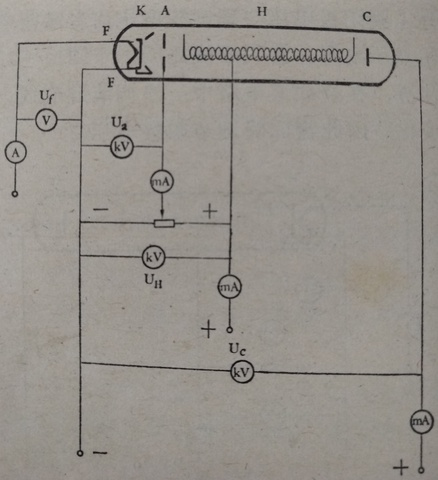
\includegraphics[width=0.52\linewidth]{figure/ch11-24}
\end{table}

\section{延长行波管寿命的措施} \label{ch12-sec4}

行波管的寿命主要决定于管子本身的质量,需要在制造管子时合理选择设计方案、制管材料及加工工艺,精心制作,提高管子质量,改进性能。但是,对于已经制成的行波管,使用、维护状况也对寿命有很大影响。这里,我们就从使用、维护的角度出发,谈谈延长行波管寿命的一些问题。

为了寻找延长行波管寿命的途径,让我们先简单分析一下管子失效的主要原因。行波管是一种比较复杂的电真空器件引起管子失效的可能因素也比较多。但是,我们从实践中知道,当前我国通信用中小功率行波管的失效,绝大多数都属于以下两种情况:

(1)电子注聚束性能变坏(即电子注散焦)。

(2)阴极发射电子能力下降。

上述两种情况都使行波管无法维持正常的直流工作状态,因而高频性能随之恶化,造成管子失效,或称寿命终了。

分析表明,这两种情况的发生,都直接与阴极性能的变化密切相关。阴极通常需要在$ \SI{750}{\degreeCelsius} \textasciitilde \SI{800}{\degreeCelsius} $的高温下才能正常工作,高温下阴极中不断发生的物理、化学变化使其发射物质逐渐减少。同时,管内残余气体对阴极的毒害;气体电离后形成的正离子对阴极的轰击;管内极间打火对阴极的伤害等等,都会使阴极性能逐渐恶化。阴极性能的变坏一种是表现为发射电流下降;另一种是阴极表面电子发射分布不均匀,破坏原来的聚束条件,引起电子注散焦。

为了延长管子的使用寿命,我们应该尽力防止阴极发射物质消耗太快,同时又要避免因管内零件过热,大量放气而恶化阴极的工作环境。下面就谈谈使用维护中应注意哪些问题,才能达到上述要求。

\subsection{严格控制灯丝电压}
对于已经制成的行波管,阴极温度高低是直接由灯丝电压的高低决定的。只有按规定数值施加灯丝电压(通常是6.3伏),阴极才在设计的温度下工作。如果温度偏高,则阴极的发射物质蒸发太快,无疑将缩短寿命。有人做过实验、发现当灯丝电压高于额定值10\%时,寿命将缩短70\%,若灯丝电压在额定值附近波动10\%,则寿命缩短50\%。阴极温度每升高$ \SI{25}{\degreeCelsius} $,发射物质的蒸发速度就约加快一倍。但是,过低的阴极温度,同样对寿命不利,因为阴极在过低的温度下更易遭受气体分子和正离子的损害而降低发射性能,所以灯丝电压也不可太低。使用中应保持在规定范围内,灯丝电压超出允许范围时应及时进行调整。
\subsection{行波管的初次启动}
行波管初次使用时应注意两点:

(1)加高压前,应先接通灯丝电压,给阴极足够的预热时间。切忌阴极尚未充分预热即接通高压。因为阴极温度低于正常值时,在高压作用下正离子的轰击更易使阴极受到伤害。这一点对于虽不是初次使用而是在关机后重新开启的行波管来说,同样是必要的。

(2)加高压前,先把阳极电压调节旋钮调至最低,收集极电压调得较高,螺旋线电压置于正常范围,然后再接通高压并调整直流工作状态至正常值。这样可以防止初次启动时螺旋线电流过大而使螺旋线过热放气,降低管内真空度。
\subsection{直流工作状态的调整}
(1)收集极电流。产品说明书中通常规定了最大允许值。使用时,根据整机、电路的实际情况,在保证高频性能的条件下,应选用尽可能低的收集极电流。这不仅可以减小收集极的消耗功率,降低温度,减少放气量,而且也有助于减轻阴极负荷及相应减小螺旋线截获电流,这些都有利于延长管子寿命。

(2)螺旋线电压。主要根据高频性能要求进行调整。但在与高频性能不发生冲突时,也应该考虑到使螺旋线电流尽可能小些。如果螺旋线电流较大,则会使螺旋线过热放气,伤害阴极,因而引起聚束情况变坏,使螺旋线电流进一步增大,这种恶性循环对管子延长寿命十分不利。

(3)收集极电压。通常应在规定的收集极电压下工作。但是,如果收集极电压适当下降并不引起螺旋线电流增加,则可在比规定值稍低的收集极电压下运用。不过,如果升高收集极电压可显著减小螺旋线电流,则宁肯在稍高于规定值的收集极电压(一般不宜超过规定值10\%)下工作。

(4)行波管电源的稳定性、可靠性对管子寿命的影响电源稳定可靠,使管子在调定的状态下稳定地工作,这无疑有利于延长行波管的使用寿命。反之,如果电源的故障频繁,将会缩短行波管的使用寿命。例如,当电源故障使收集极电压大大降低甚至趋于零,则管内电子流将全部打在螺旋线上,引起大量放气,使管内真空度变坏或者把螺旋线轰断,使管子无法工作;又如阳极电压因电源故障而突然升高,则收集极电流、螺旋线电流也将同时增加,引起收集极和螺旋线的放气,降低管内真空度;再如螺旋线电压因故障而偏离规定范围造成散焦也会降低管内真空度等等。所有这些原因都会缩短管子的寿命。
\subsection{行波管与散热装置应接触良好,以便充分发挥散热能力,降低行波管工作温度}

在高温环境下,如果发现行波管散热不良,若能利用辅助散热手段,帮助提高散热效果,那么对延长管子寿命也是有利的

\subsection{必要时开启管内钛泵}

有的行波管内设有辅助吸气装置钛泵,按说明书规定的方法使钛泵工作,可提高管内真空度,这对改善阴极工作环境改善管子的聚束性能及噪声性能,因而延长管子的使用寿命都是有利的。
\begin{figure}[phtb]
	\centering
	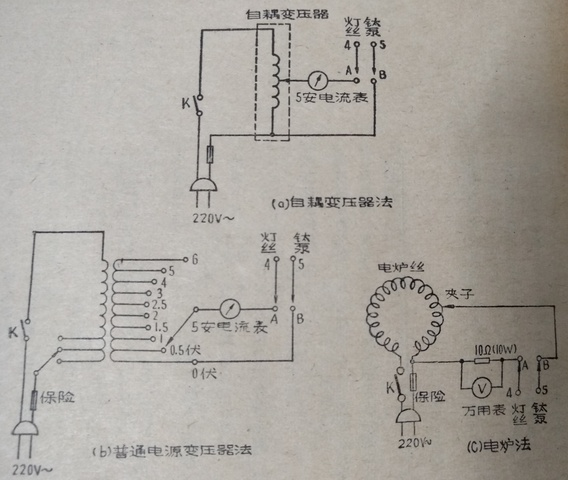
\includegraphics[width=0.52\linewidth]{figure/ch12-1}
	\caption{烧钛泵示意图}
	\label{ch12-1}
\end{figure}
\subsection{延长行波管寿命的特殊措施}
(1)调整聚束系统,改善聚束性能。对于因散焦而失效的管子,如果有条件,可将包装体拆开,重新调整聚束磁场上的磁补偿零件,使磁场分布适应于失效管子内部发生的变化,聚束性能往往可以得到不同程度的恢复,行波管就可以继续使用当然,这个工作不仅需要有相应的电源设备,同时需要操作者经过适当的训练,掌握聚束的调整方法。

(2)提高阴极工作温度。对于经过长期使用后阴极发射能力显著降低,或者聚束性能显著变坏的行波管,可试将灯丝电压调整为正常值的1.1\textasciitilde1.2倍,例如由6.3伏增加至7\textasciitilde7.5伏以提高阴极发射能力,可使部分失效行波管的发射电流或聚束性能得到改善,因而可以继续工作一段时间。当然,由于阴极在过高温度下发射物质更快地消耗,所以这样的管子继续工作的时间是有限的。

最后,需要说明一点,在本章中我们对行波管的调整、使用以及延长寿命等问题分别作了一些介绍。由于是从不同的角度来介绍的(如第\ref{ch12-sec4}节是专门从寿命的角度来介绍的),因而有些内容有重复的现象。但为了保持每个专题的系统性,我们仍然保留了这些重复的部分。

